% Week 9 report, Project 1. IEEE conference class when available (Overleaf), else a
% two-column article with the same layout.
\IfFileExists{IEEEtran.cls}{\documentclass[conference]{IEEEtran}}{%
  \documentclass[10pt,twocolumn,a4paper]{article}
  \usepackage[margin=17mm,columnsep=6mm]{geometry}
  \usepackage{mathptmx}}
\usepackage{amsmath,amssymb,booktabs,graphicx,xcolor}
\usepackage[hidelinks]{hyperref}
\usepackage[numbers,sort&compress]{natbib}
\setlength{\abovedisplayskip}{4pt}\setlength{\belowdisplayskip}{4pt}
\newcommand{\NUMwithinAcc}{84.3\%}
\newcommand{\NUMcrossAcc}{90.3\%}
\newcommand{\NUMwithinCost}{0.244}
\newcommand{\NUMcrossCost}{0.168}
\newcommand{\NUMoverallSentence}{Both learned models beat the majority baseline by a wide margin (type-weighted cost 1.11 for the majority class against 0.24 for logistic regression and 0.23 for the forest on held-out female types). On the male brain they score \emph{better}, not worse: logistic regression costs $0.168\pm0.025$ against $0.244\pm0.017$, with the same sign at $\tau=5$ (0.157 vs 0.211) and $\tau=15$ (0.205 vs 0.302). Re-weighting by \texttt{class\_weight="balanced"} raises balanced accuracy from 60\% to 75\% but nearly doubles the expected cost (0.244 to 0.431).}
\newcommand{\NUMregionSentence}{Every region looks cheaper on the male brain. Part of this is composition: held-out female types without a male match are harder, and restricting the female side to matched types shrinks the overall gap from $-0.076\pm0.015$ to $-0.022\pm0.011$. Part is measurement: the male graph is more complete (8,639 against 14,810 isolated neurons at the scaled thresholds). Higher-order centres are the cheapest region in both brains (0.071 female, 0.052 male, matched types) because nearly all their neurons are \texttt{central}; they improve slightly ($-0.019\pm0.007$; bootstrap over types $[-0.039,-0.024]$ against all held-out types) while their floor is $0.002\pm0.002$. The only positive drop, in the optic lobe ($+0.034\pm0.042$), lies within one SD of zero and of its floor ($0.017\pm0.024$). The naive analysis therefore shows no degradation concentrated in higher-order centres.}
\newcommand{\NUMfigOneCaption}{Light bars: the pre-registered comparison with all held-out female types; dark bars: female side restricted to types with a male match.}
\newcommand{\NUMunmatchedSentence}{The 7,177 male neurons with no FAFB type (no \texttt{flywire\_type}, or one that names no FAFB type; the 3,275 of the feedback are only the first group) are scored by all 15 fold models: type-weighted cost $0.219\pm0.031$, against 0.219 for female held-out neurons of the same super\_class $\times$ region cells (98.8\% of them covered), so no drop. The 1,227 male-specific neurons among them are labelled correctly in 98.4\% of cases (cost 0.030): at the super\_class level they are mostly \texttt{central}.}
\newcommand{\NUMefferentSentence}{The 16 efferent neurons, a class never seen in training, are always wrong (80 predictions by the five seed-0 fold models: optic 34, sensory 26, central 10, ascending 10; mean cost 3.66), almost half of them into the afferent flow.}
\newcommand{\NUMdimSentence}{Matched sexually dimorphic types (about 135 neurons per fold) show no reliable change ($-0.034\pm0.143$).}
\newcommand{\NUMsensoryShift}{16,904 sensory neurons in FAFB against 8,918 in the MaleCNS brain part; R1-6 photoreceptors 8,452 against 0}
\newcommand{\NUMevidenceSentence}{For plain logistic regression the cost-minimising rule changes only 0.27\% of type-weighted decisions and the cost from 0.1676 to 0.1672: its probabilities are confident, so here $\arg\max$ is nearly the cheapest choice, a negative finding on this axis. For the class-weighted model the rule changes 2.8\% of decisions (8.3\% in the motor periphery) and saves about 0.046 per type (0.380 to 0.334, 12\%), mostly in the sensory and motor periphery, where input and output classes compete, as (c)--(d) predict. The larger failure is the class-weighted fit itself: per-class weights trade expected cost for balanced accuracy (cost 0.244 to 0.431 while balanced accuracy goes from 60\% to 75\%), the gap of (b).}
\newcommand{\NUMpriorSentence}{The EM prior correction, which uses no male label, makes the cost worse (0.168 to 0.184), as expected when whole types are missing rather than class shares shifting within the same types: the 8,452 R1-6 photoreceptors of FAFB are absent from the male brain part, and 1,742 male neurons are assigned to the lamina against 9,486 female.}
\newcommand{\NUMfigThreeCaption}{Plain logistic regression (blue) barely changes; the class-weighted model (red) saves most where afferent and efferent classes compete.}


\title{Where connectivity-based cell typing fails:\\ a naive cross-sex baseline and why it does not answer the question}
\author{Y{\i}lmaz B\"uy\"uk (263031030001)\\ Connectome course, Project 1 --- Week 9 milestone\\
\small Code: \url{https://github.com/yilmazbuyuk/connectome-project1} (tag \texttt{week9})}
\date{}

\begin{document}
\maketitle

\begin{abstract}
Connectivity identifies cell type, but published evaluations count every confusion as equally bad and test within one animal. We ask which cell types a connectivity classifier gets wrong under a biologically motivated cost matrix when it is trained on the female brain (FlyWire FAFB) and tested on the male brain (MaleCNS), and whether the errors concentrate in higher-order centres. Off-the-shelf multinomial logistic regression and a random forest reach \NUMwithinAcc{} type-weighted accuracy on held-out female cell types and \NUMcrossAcc{} on the same types in the male brain, at an expected cost of \NUMwithinCost{} and \NUMcrossCost{} per type: the male test is not harder, and no region, higher-order centres included, degrades beyond a within-animal noise floor. We derive why this answer is not the one the question needs: a per-class weight cannot express a cost that depends on the predicted class, the most probable class is not the cheapest one, and a classifier trained under the female class mix carries the wrong prior to the male test set.
\end{abstract}

% ======================================================================
\section{Naive result}

\paragraph{Context} Connectivity alone identifies cell type \citep{ntac,schlegel2024}; the open question is which confusions are costly and whether they concentrate where the sexes differ, mostly in higher-order centres \citep{berg2026}. Proofreading and synapse detection differ between the two volumes \citep{dorkenwald2024}, so not every cross-dataset change is a sex effect.

\paragraph{Set-up (lock note v2)} One sample is one neuron; the label $y$ is its corrected \texttt{super\_class} (10 levels shared by both datasets); the features $x$ are connectivity only: all-synapse input and output totals (MaleCNS divided by 1.484, the matched-type synapse ratio), in- and out-degree at the locked threshold, and the share of input and output synapses in each of 44 neuropils (left and right merged) plus an unassigned column, 100 features in all (lock: Features, Cross-dataset). Edges count at $\tau=10$ synapses in FAFB and $\tau=15$ in MaleCNS (lock: Threshold). Folds hold out whole cell types, with matched MaleCNS types in the same fold as their FAFB type: 5 folds $\times$ seeds 0, 1, 2 = 15 splits (lock: Split). In every split the model is trained on the FAFB training types and scored on the held-out FAFB types (\emph{within-sex}) and on the MaleCNS neurons of the same held-out types (\emph{cross-sex}); the difference is the \emph{drop}. Hyperparameters are tuned inside the training folds by grouped 3-fold cross-validation on log-loss (LR: $C\in\{0.01,0.1,1,10\}$; RF: 500 trees, min.\ leaf size $\in\{1,5,20\}$). Every metric is reported type-weighted (each neuron weighted by $1/$its type size), the headline, and neuron-weighted (lock: Metric weighting). The cost matrix $C$ follows information flow \citep{schlegel2024}: 0 on the diagonal, 1 within a flow, 2 between intrinsic and afferent or efferent, 5 between afferent and efferent.

\paragraph{Baseline and naive models} Table~\ref{tab:overall} compares the majority class, multinomial logistic regression with and without \texttt{class\_weight="balanced"} and a random forest. \NUMoverallSentence{}

\begin{table*}[t]\centering\footnotesize
\caption{Naive results, $\tau=10$, mean $\pm$ SD over 15 splits (5 grouped folds $\times$ 3 seeds). F = held-out female types (within-sex), M = the same types in the male brain (cross-sex). Cost = mean locked flow cost per neuron (0 = all correct); accuracy, macro-F1 and balanced accuracy in \%. Top block type-weighted (headline), bottom block neuron-weighted.}
\label{tab:overall}
\begin{tabular}{@{}l cc cc cc cc@{}}\toprule
 & \multicolumn{2}{c}{Expected cost $\downarrow$} & \multicolumn{2}{c}{Accuracy} & \multicolumn{2}{c}{Macro-F1} & \multicolumn{2}{c}{Balanced acc.}\\
\cmidrule(lr){2-3}\cmidrule(lr){4-5}\cmidrule(lr){6-7}\cmidrule(lr){8-9}
Model & F & M & F & M & F & M & F & M\\\midrule
\multicolumn{9}{@{}l}{\emph{type-weighted}}\\
Majority & 1.113$\pm$0.012 & 1.107$\pm$0.013 & 8.4$\pm$0.5 & 3.0$\pm$0.3 & 1.6$\pm$0.1 & 0.6$\pm$0.1 & 10.0$\pm$0.0 & 11.0$\pm$0.4\\
LogReg & 0.244$\pm$0.017 & 0.168$\pm$0.025 & 84.3$\pm$1.0 & 90.3$\pm$1.4 & 60.6$\pm$4.4 & 63.4$\pm$7.8 & 60.1$\pm$4.9 & 60.4$\pm$7.2\\
LogReg bal. & 0.431$\pm$0.018 & 0.380$\pm$0.034 & 76.4$\pm$1.3 & 78.9$\pm$1.9 & 55.4$\pm$2.1 & 55.2$\pm$4.5 & 74.5$\pm$2.9 & 69.5$\pm$5.9\\
Random forest & 0.231$\pm$0.013 & 0.173$\pm$0.018 & 85.4$\pm$0.7 & 90.3$\pm$0.9 & 59.0$\pm$2.8 & 62.3$\pm$5.6 & 56.3$\pm$2.7 & 56.9$\pm$4.7\\
\midrule
\multicolumn{9}{@{}l}{\emph{neuron-weighted}}\\
Majority & 0.592$\pm$0.211 & 0.437$\pm$0.089 & 55.7$\pm$10.6 & 64.8$\pm$6.4 & 7.1$\pm$0.9 & 8.6$\pm$0.5 & 10.0$\pm$0.0 & 11.0$\pm$0.4\\
LogReg & 0.149$\pm$0.077 & 0.137$\pm$0.068 & 90.8$\pm$4.1 & 92.0$\pm$3.5 & 63.9$\pm$5.0 & 63.5$\pm$8.5 & 60.1$\pm$5.2 & 58.3$\pm$8.8\\
LogReg bal. & 0.260$\pm$0.125 & 0.246$\pm$0.107 & 83.3$\pm$7.2 & 83.1$\pm$6.2 & 50.8$\pm$2.5 & 52.4$\pm$4.3 & 75.0$\pm$2.8 & 71.5$\pm$7.5\\
Random forest & 0.153$\pm$0.121 & 0.143$\pm$0.081 & 90.8$\pm$6.3 & 91.5$\pm$4.1 & 61.7$\pm$3.9 & 61.5$\pm$7.3 & 56.0$\pm$3.7 & 54.4$\pm$6.4\\
\bottomrule\end{tabular}\end{table*}

\paragraph{Where the drop falls} Fig.~\ref{fig:headline} splits the cross-sex drop by the anatomical region group of each neuron, fixed from the neuropil table before any model was run (lock: Region grouping; the A7 observation was not used). The black diamonds are a within-animal noise floor: the same models trained on one FAFB hemisphere and tested on the held-out types of the other. \NUMregionSentence{}

\begin{figure}[t]\centering
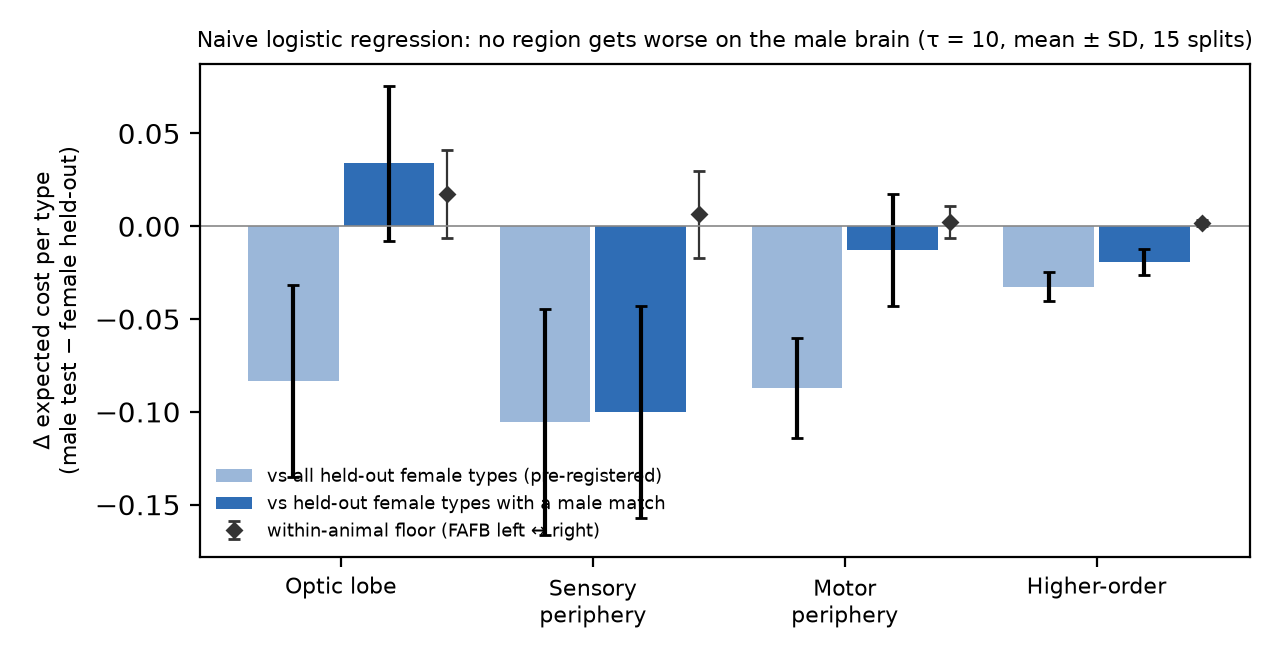
\includegraphics[width=\columnwidth]{../figures/week9/fig1_headline_drop_by_region.png}
\caption{Cross-sex drop in type-weighted expected cost by region group (bars; mean $\pm$ SD over 15 splits). Look at whether the bars rise above the within-animal floor (diamonds), and whether they are highest in higher-order centres as the dimorphism results predict. \NUMfigOneCaption{}}
\label{fig:headline}
\end{figure}

\paragraph{Unmatched, efferent and dimorphic neurons} \NUMunmatchedSentence{} \NUMefferentSentence{} \NUMdimSentence{}

% ======================================================================
\section{Why the naive answer is not the answer}

\paragraph{Notation} Classes $k=1,\dots,K$ ($K=10$); $x\in\mathbb{R}^d$; $W=[w_1,\dots,w_K]$ with intercepts absorbed; logits $z_k=w_k^\top x$; $p_k(x)=e^{z_k}/\sum_m e^{z_m}$. $C(j,k)\ge 0$ is the cost of predicting $k$ when the truth is $j$, with $C(j,j)=0$. $P_S(j\mid x)$ and $\pi^S_j$ are the posterior and the class prior in dataset $S\in\{F,M\}$ (female, male).

\paragraph{1. The target} The question asks for the expected cost of a decision rule $h$ on the male brain, by region group $g$:
\begin{equation}
R^M_g(h)=\mathbb{E}_{(x,y)\sim M}\big[\,C(y,h(x))\mid \text{region}=g\,\big],
\label{eq:target}
\end{equation}
with the expectation taken over cell types (type-weighted), compared with the same quantity on held-out female types. For fixed $x$ the rule that minimises \eqref{eq:target} is
\begin{equation}
h^\star(x)=\arg\min_k\; \sum_{j} C(j,k)\,P_M(j\mid x).
\label{eq:bayes}
\end{equation}

\paragraph{2. What the naive method computes} scikit-learn's multinomial \texttt{LogisticRegression} (solver \texttt{lbfgs}) solves \citep{sklearn}
\begin{equation}
\hat W=\arg\min_W\; \tfrac12\lVert W\rVert_F^2 \;+\; C_{\text{reg}}\sum_{i=1}^n a_{y_i}\,\big(-\log p_{y_i}(x_i)\big),
\label{eq:naive}
\end{equation}
where the L2 penalty is on by default (intercepts unpenalised), $C_{\text{reg}}$ is its inverse strength and $a_j$ is the class weight: $a_j=1$ by default, $a_j=n/(K n_j)$ for \texttt{"balanced"}. It then predicts $\hat y=\arg\max_k p_k(x)$. The random forest also predicts the class with the largest averaged vote. Neither sees $C$, and both are fitted on FAFB, so they estimate $P_F$, not $P_M$.

\paragraph{3. The gap, derived} \emph{(a) Gradients.} For one example of class $j$, with $\partial p_k/\partial z_m = p_k(\mathbb{1}[k{=}m]-p_m)$, the gradient of the weighted log-loss in \eqref{eq:naive} is
\begin{equation}
\nabla_{w_m}\big(-a_j\log p_j\big)= a_j\,\big(p_m(x)-\mathbb{1}[m=j]\big)\,x .
\label{eq:gradce}
\end{equation}
The expected-cost loss of the brief, $L(x,j)=\sum_k C(j,k)p_k(x)$, has instead
\begin{equation}
\nabla_{w_m}L= p_m(x)\Big(C(j,m)-\sum_k C(j,k)\,p_k(x)\Big)\,x
\label{eq:gradcost}
\end{equation}
(derivation in Appendix~A). In \eqref{eq:gradce} the weight $a_j$ multiplies the whole vector and depends only on the true class; in \eqref{eq:gradcost} the push on logit $m$ depends on $C(j,m)$, i.e.\ on the true \emph{and} the predicted class.

\emph{(b) What the weighted fit converges to.} With enough data and a flexible enough model, the minimiser of the expected weighted log-loss at $x$ solves $\min_q -\sum_j a_jP(j\mid x)\log q_j$ subject to $\sum_j q_j=1$. A Lagrange multiplier gives
\begin{equation}
q_j(x)=\frac{a_j\,P(j\mid x)}{\sum_m a_m P(m\mid x)},\qquad \arg\max_k q_k = \arg\max_k a_kP(k\mid x).
\label{eq:qstar}
\end{equation}
\emph{(c) The decision boundaries cannot match.} Under \eqref{eq:qstar} the boundary between classes $k$ and $l$ is $a_kP_k=a_lP_l$: it involves only $P_k$ and $P_l$. Under \eqref{eq:bayes} it is $\sum_j\big(C(j,k)-C(j,l)\big)P_j=0$. For our matrix and $k$ = sensory, $l$ = motor this is
\begin{equation}
5\,(P_{\text{mot}}-P_{\text{sen}})+4\,\big(P_{\text{desc}}+P_{\text{endo}}-P_{\text{asc}}-P_{\text{sasc}}\big)=0,
\label{eq:boundary}
\end{equation}
because intrinsic classes cost 2 under both predictions and cancel (Appendix~B). The boundary depends on the probabilities of \emph{other} classes (ascending, descending, \dots), which no choice of $a$ can reproduce. So no class weighting makes the naive rule cost-optimal for this $C$.

\emph{(d) Worked example.} Let the model give sensory 0.45, central 0.15, motor 0.40. The naive rule predicts sensory. The expected costs under our $C$ are
sensory $0.15\cdot2+0.40\cdot5=2.30$, central $0.45\cdot2+0.40\cdot2=1.70$, motor $0.45\cdot5+0.15\cdot2=2.55$:
the cheapest answer is the \emph{least} probable class, the intrinsic class that sits between input and output (with the 1/2/10 matrix: 4.30, 1.70, 4.80). With the illustrative costs of the brief (missing sensory 10, intrinsic called sensory 2, central/optic 1) and $p=(0.40,0.25,0.35)$ for central, optic, sensory, the naive rule picks central (3.75) while sensory costs 1.30.

\emph{(e) The prior travels with the model.} If $P(x\mid j)$ were the same in both brains (pure label shift), Bayes' rule gives $P_M(j\mid x)\propto P_F(j\mid x)\,\pi^M_j/\pi^F_j$, so a model fitted on FAFB uses the female prior on the male test set \citep{elkan2001}. Here the shift is large for sensory neurons (\NUMsensoryShift{}), mostly because the male lamina and its photoreceptors are only partly inside the volume \citep{nern2025}. That removes whole types, so it is not a pure label shift; we report an EM prior correction \citep{saerens2002} that uses no test label only as a check.

\paragraph{4. When they coincide} (i) Unit costs $C(j,k)=\mathbb{1}[j\ne k]$: $\sum_{j\ne k}P_j=1-P_k$, so \eqref{eq:bayes} is $\arg\max_kP_k$, the naive rule. (ii) Costs that depend only on the true class, $C(j,k)=c_j$ for $j\ne k$: $\sum_{j\ne k}c_jP_j=\text{const}-c_kP_k$, so the optimum is $\arg\max_k c_kP_k$, which \eqref{eq:qstar} reaches with $a_j=c_j$ in the large-sample limit. (iii) No prior shift, $\pi^M=\pi^F$. Case (i) is the verification target of the week~11 implementation.

\paragraph{5. The evidence} The derivation predicts that, with the \emph{same} naive probabilities, replacing $\arg\max$ by \eqref{eq:bayes} lowers the cost, most where the model is torn between flows. \NUMevidenceSentence{} (Fig.~\ref{fig:rule}.) \NUMpriorSentence{}

\begin{figure}[t]\centering
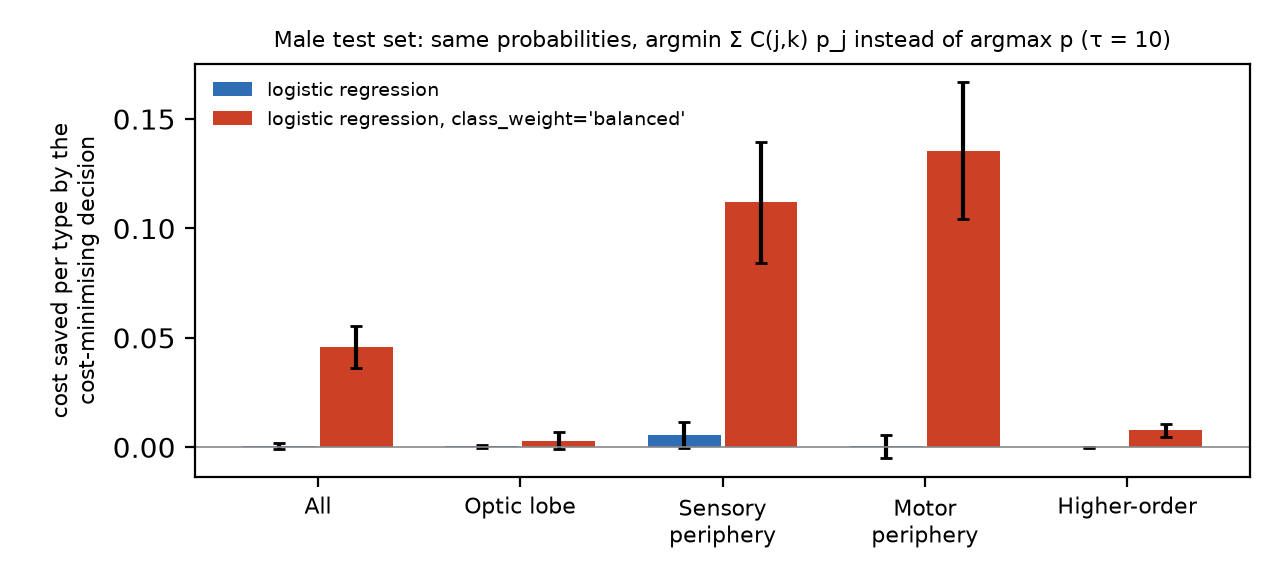
\includegraphics[width=\columnwidth]{../figures/week9/fig3_decision_rule.png}
\caption{Same logistic-regression probabilities on the male test set, two decision rules. The gap between the bars is what the decision rule alone costs; it is a diagnostic of the derivation, not the week~11 model. \NUMfigThreeCaption{}}
\label{fig:rule}
\end{figure}

\paragraph{What the fix must do} The week~11 model must (1) learn probabilities that are calibrated under the training distribution, from an objective in which the cost of a mistake depends on both the true and the predicted class, as in \eqref{eq:gradcost}; (2) decide with \eqref{eq:bayes}, not $\arg\max$; (3) state how the test prior enters without test labels; and (4) reproduce scikit-learn's multinomial logistic regression in case (i), checked together with a finite-difference gradient check. Whether the drop is a sex effect is decided against the between-animal floor (FAFB$\to$hemibrain), also due in week~11.

{\footnotesize
\begin{thebibliography}{9}
\bibitem{schlegel2024} P.~Schlegel \emph{et al.}, ``Whole-brain annotation and multi-connectome cell typing of \emph{Drosophila},'' \emph{Nature}, 634, 2024.
\bibitem{sklearn} scikit-learn developers, ``LogisticRegression'' and ``RandomForestClassifier,'' scikit-learn 1.x API documentation, 2025.
\bibitem{elkan2001} C.~Elkan, ``The foundations of cost-sensitive learning,'' in \emph{Proc. IJCAI}, 2001.
\bibitem{saerens2002} M.~Saerens, P.~Latinne, C.~Decaestecker, ``Adjusting the outputs of a classifier to new a priori probabilities,'' \emph{Neural Computation}, 14(1), 2002.
\bibitem{nern2025} A.~Nern \emph{et al.}, ``Connectome-driven neural inventory of a complete visual system,'' \emph{Nature}, 2025.
\bibitem{dorkenwald2024} S.~Dorkenwald \emph{et al.}, ``Neuronal wiring diagram of an adult brain,'' \emph{Nature}, 634, 2024.
\bibitem{berg2026} S.~Berg \emph{et al.}, ``Sexual dimorphism in the complete connectome of the \emph{Drosophila} male central nervous system,'' \emph{Cell}, 2026.
\bibitem{ntac} NTAC preprint, connectivity-based cell typing, 2025.
\end{thebibliography}}

\appendix
\section*{Appendix A: gradient of the expected-cost loss}
$L=\sum_kC(j,k)p_k$. With $\partial p_k/\partial z_m=p_k(\mathbb{1}[k{=}m]-p_m)$,
\begin{align*}
\frac{\partial L}{\partial z_m}&=\sum_kC(j,k)p_k\mathbb{1}[k{=}m]-p_m\sum_kC(j,k)p_k\\
&=p_m\Big(C(j,m)-\sum_kC(j,k)p_k\Big),
\end{align*}
and $\partial z_m/\partial w_m=x$. For the weighted log-loss, $-a_j\log p_j$: $\partial/\partial z_m=-a_j(\mathbb{1}[j{=}m]-p_m)=a_j(p_m-\mathbb{1}[m{=}j])$. Adding $\tfrac{1}{2C_{\text{reg}}}\lVert W\rVert_F^2$ (per-sample scaling of \eqref{eq:naive}) adds $w_m/C_{\text{reg}}$ to every gradient and shrinks all logits towards zero, which pulls $p$ towards uniform.

\section*{Appendix B: the sensory--motor boundary}
$\Delta_j=C(j,\text{sen})-C(j,\text{mot})$. Truth sensory: $0-5=-5$. Truth motor: $5-0=5$. Truth ascending or sensory\_ascending (afferent): $1-5=-4$. Truth descending or endocrine (efferent): $5-1=4$. Truth optic, central, visual\_projection, visual\_centrifugal (intrinsic): $2-2=0$. So $\sum_j\Delta_jP_j=5(P_{\text{mot}}-P_{\text{sen}})+4(P_{\text{desc}}+P_{\text{endo}}-P_{\text{asc}}-P_{\text{sasc}})$.

\section*{Appendix C: lock note v2 items in force}
{\footnotesize
\begin{tabular}{@{}p{0.27\columnwidth}p{0.68\columnwidth}@{}}
\toprule
Item & Choice (lock note v2, unchanged; no deviation)\\
\midrule
Target & \texttt{super\_class}, 10 levels; \texttt{unknown} out; MaleCNS \texttt{efferent} (16) scored apart\\
Split & whole types held out; 5 folds $\times$ seeds 0,1,2; key FAFB \texttt{cell\_type} = MaleCNS \texttt{flywire\_type}; splits in \texttt{reports/week9\_splits.csv}\\
Threshold & FAFB $\tau=10$; sensitivity 5, 15 (seed 0)\\
Cross-dataset & MaleCNS $\tau=\mathrm{round}(1.484\,\tau)$; totals $\div 1.484$\\
Features & $n_{\text{in}}, n_{\text{out}}$ (all synapses / brain-part connections), degrees, 2$\times$45 neuropil shares; L/R merged\\
Population & all brain neurons (FAFB 139,255; MaleCNS 144,414)\\
Missing values & no input/output: shares 0, degree 0, flags\\
Region & shared alphabetical ties; 4 anatomical groups\\
Weighting & type-weighted headline; neuron-weighted beside\\
Prior shift & unadjusted headline; EM priors as check\\
Floor & FAFB left$\leftrightarrow$right, same folds\\
Tuning & inner grouped 3-fold CV on log-loss; RF tuned with 100 trees, refit with 500\\
\bottomrule
\end{tabular}}


\end{document}
